\documentclass[]{article}
\usepackage[T1]{fontenc}
\usepackage{lmodern}
\usepackage{amssymb,amsmath}
\usepackage{ifxetex,ifluatex}
\usepackage{fixltx2e} % provides \textsubscript
% use microtype if available
\IfFileExists{microtype.sty}{\usepackage{microtype}}{}
\ifnum 0\ifxetex 1\fi\ifluatex 1\fi=0 % if pdftex
  \usepackage[utf8]{inputenc}
\else % if luatex or xelatex
  \usepackage{fontspec}
  \ifxetex
    \usepackage{xltxtra,xunicode}
  \fi
  \defaultfontfeatures{Mapping=tex-text,Scale=MatchLowercase}
  \newcommand{\euro}{€}
\fi
\usepackage{color}
\usepackage{fancyvrb}
\DefineShortVerb[commandchars=\\\{\}]{\|}
\DefineVerbatimEnvironment{Highlighting}{Verbatim}{commandchars=\\\{\}}
% Add ',fontsize=\small' for more characters per line
\newenvironment{Shaded}{}{}
\newcommand{\KeywordTok}[1]{\textcolor[rgb]{0.00,0.44,0.13}{\textbf{{#1}}}}
\newcommand{\DataTypeTok}[1]{\textcolor[rgb]{0.56,0.13,0.00}{{#1}}}
\newcommand{\DecValTok}[1]{\textcolor[rgb]{0.25,0.63,0.44}{{#1}}}
\newcommand{\BaseNTok}[1]{\textcolor[rgb]{0.25,0.63,0.44}{{#1}}}
\newcommand{\FloatTok}[1]{\textcolor[rgb]{0.25,0.63,0.44}{{#1}}}
\newcommand{\CharTok}[1]{\textcolor[rgb]{0.25,0.44,0.63}{{#1}}}
\newcommand{\StringTok}[1]{\textcolor[rgb]{0.25,0.44,0.63}{{#1}}}
\newcommand{\CommentTok}[1]{\textcolor[rgb]{0.38,0.63,0.69}{\textit{{#1}}}}
\newcommand{\OtherTok}[1]{\textcolor[rgb]{0.00,0.44,0.13}{{#1}}}
\newcommand{\AlertTok}[1]{\textcolor[rgb]{1.00,0.00,0.00}{\textbf{{#1}}}}
\newcommand{\FunctionTok}[1]{\textcolor[rgb]{0.02,0.16,0.49}{{#1}}}
\newcommand{\RegionMarkerTok}[1]{{#1}}
\newcommand{\ErrorTok}[1]{\textcolor[rgb]{1.00,0.00,0.00}{\textbf{{#1}}}}
\newcommand{\NormalTok}[1]{{#1}}
% Redefine labelwidth for lists; otherwise, the enumerate package will cause
% markers to extend beyond the left margin.
\makeatletter\AtBeginDocument{%
  \renewcommand{\@listi}
    {\setlength{\labelwidth}{4em}}
}\makeatother
\usepackage{enumerate}
\usepackage{graphicx}
% We will generate all images so they have a width \maxwidth. This means
% that they will get their normal width if they fit onto the page, but
% are scaled down if they would overflow the margins.
\makeatletter
\def\maxwidth{\ifdim\Gin@nat@width>\linewidth\linewidth
\else\Gin@nat@width\fi}
\makeatother
\let\Oldincludegraphics\includegraphics
\renewcommand{\includegraphics}[1]{\Oldincludegraphics[width=\maxwidth]{#1}}
\ifxetex
  \usepackage[setpagesize=false, % page size defined by xetex
              unicode=false, % unicode breaks when used with xetex
              xetex]{hyperref}
\else
  \usepackage[unicode=true]{hyperref}
\fi
\hypersetup{breaklinks=true,
            bookmarks=true,
            pdfauthor={},
            pdftitle={},
            colorlinks=true,
            urlcolor=blue,
            linkcolor=magenta,
            pdfborder={0 0 0}}
\setlength{\parindent}{0pt}
\setlength{\parskip}{6pt plus 2pt minus 1pt}
\setlength{\emergencystretch}{3em}  % prevent overfull lines
\setcounter{secnumdepth}{0}

\author{}
\date{}

\begin{document}

\section{Bios301 Final Exam}

\textbf{\emph{2013-12-12}}

Please answer \textbf{any three} of the four questions below (if you
submit answers to all four, only the first three will be graded). You
may use any static reference materials you wish, but \textbf{no
collaboration or consultation with any individual or service is
permitted}. The instructor will answer any clarifying or technical
questions you may have (email to chris.fonnesbeck@vanderbilt.edu or
call/text to 615-955-0380). This exam is subject to the
\href{http://www.vanderbilt.edu/student\_handbook/the-honor-system\#honorcode}{Vanderbilt
University honor code}.

The completed exam is due \textbf{Friday, Dec. 13 by Noon CST}. Your
exam should be pushed to the private GitHub repository that you have
been using to submit homework assignments. Please create a separate
folder called \texttt{exam} to contain all exam materials. No content
outside this directory will be considered when grading the exam. Content
checked in after Noon on Dec. 13 will not be graded.

To obtain full marks, you must:

\begin{enumerate}[1.]
\item
  Submit working code to generate answers to all questions. Please test
  your code before submitting to ensure that it runs cleanly.
\item
  Completely annotate your code and your results in order to fully
  explain what you have done, and what the output means. It should be
  readable by a non-R user.
\item
  Submit a knitr file in either \texttt{.rnw} or \texttt{.rmd} format,
  along with its output (LaTeX or Markdown, respectively).
\end{enumerate}

\subsection{Question 1}

\textbf{25 points}

\begin{enumerate}[a.]
\item
  Write a function \texttt{eval\_poly} which will evaluate and return
  polynomials of the form:
\end{enumerate}

\[P(x) = c_n x^{n−1} + c_{n−1} x^{n−2} + \ldots + c_2 x + c_1\]

The arguments of the function should include $x$ and the vector of
polynomial coefficients $c = [c_1, \ldots, c_n]$.

\begin{enumerate}[a.]
\setcounter{enumi}{1}
\item
  For moderate to large values of n, evaluation of a polynomial at x can
  be done more efficiently using Horner's Rule:
\end{enumerate}

\begin{enumerate}[1.]
\item
  Set $a_n \leftarrow c_n$.
\item
  For $i=n−1,\ldots,1$ set $a_i = a_{i+1} x+c_i$.
\item
  Return $a_1$. (This is the computed value of $P(x)$).
\end{enumerate}

Write an R function with arguments x and a vector of polynomial
coefficients and which returns the value of the polynomial evaluated at
x. Ensure that your function returns an appropriate vector of values
when x is a vector.

\begin{enumerate}[a.]
\setcounter{enumi}{2}
\item
  Do some timings to compare the algorithms used in the previous two
  questions. In particular, try the following code:
\end{enumerate}

\begin{Shaded}
\begin{Highlighting}[]
\KeywordTok{system.time}\NormalTok{(}\KeywordTok{eval_poly}\NormalTok{(}\DataTypeTok{x=}\KeywordTok{seq}\NormalTok{(-}\DecValTok{10}\NormalTok{, }\DecValTok{10}\NormalTok{, }\DataTypeTok{length=}\DecValTok{500000}\NormalTok{), }\KeywordTok{c}\NormalTok{(}\DecValTok{1}\NormalTok{,-}\DecValTok{2}\NormalTok{,}\DecValTok{2}\NormalTok{,}\DecValTok{3}\NormalTok{,}\DecValTok{4}\NormalTok{,}\DecValTok{6}\NormalTok{,}\DecValTok{7}\NormalTok{)))}
\end{Highlighting}
\end{Shaded}

and compare it to a similar call to the function in part (b).

\begin{enumerate}[a.]
\setcounter{enumi}{3}
\item
  What happens to the comparison when the number of polynomial
  coefficients is smaller? Try the polynomial:
\end{enumerate}

\[P(x) = 2x^{2} +17x−3\]

\subsection{Question 2}

\textbf{25 points}

Estimate the coverage probability of 95\% bootstrap percentile intervals
for the binomial probability \texttt{p} in the following model:

\[x \sim \text{Binomial}(n=20, p=0.3)\]

Is this interval conservative, unbiased, or liberal?

\subsection{Question 3}

\textbf{25 points}

The central limit theorem claims that if X is a Poisson random variable
with parameter λ, and

\[Z = \frac{X-\lambda}{\sqrt{\lambda}}\]

then Z is approximately standard normal (\emph{i.e.} $N(0,1)$), and the
approximation improves as λ gets large.

\begin{enumerate}[a.]
\item
  Write code to simulate a large number of Z values for values of λ in
  the set $\\{1,3,5,\ldots,99\\}$. Execute the code and describe how the
  distribution of Z changes as λ increases.
\item
  Write a function in ggplot2 that generates a series of QQ-plots, which
  plots the \emph{calculated} values of Z against their
  \emph{theoretical} values under a true standard normal, along with a
  diagonal that represents perfect correspondence between the actual and
  theoretical values. Use this code to generate QQ-plots for the results
  in part (a). An individual plot should similar to this:
\end{enumerate}

\begin{figure}[htbp]
\centering
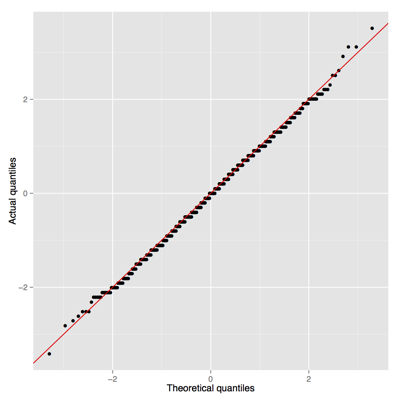
\includegraphics{qqplot.png}
\caption{qqplot}
\end{figure}

You will probably need to plot a few multi-plot panels so that your
graphs are readable.

Hint: to get theoretical quantiles corresponding to Z, use the following
code:

\begin{verbatim}
qnorm(ppoints(length(z)))[order(order(z))]
\end{verbatim}

\begin{enumerate}[a.]
\setcounter{enumi}{2}
\item
  Based on your plots, about how large must λ be before the
  approximation becomes reasonable? Here ``reasonable'' means that it is
  appropriate to make normality assumptions with the sample.
\end{enumerate}

\subsection{Question 4}

\textbf{25 points}

In order to explore how home run hitting in baseball has changed
throughout history, let's create a data visualization using the
\texttt{baseball-databank} database.

Use the data in the \texttt{Batting} table to create a plot of home run
rate by team across years. We will use home run rate to account for
differing numbers of at-bats (AB) among players and teams:

\[HRRate = HR/AB\]

So, this quantity expresses the probability of hitting a home run in any
given at bat.

Your solution must include the following:

\begin{enumerate}[a.]
\item
  Connect to the \texttt{baseball-databank} database using
  \texttt{RSQLite} in order to query from the \texttt{Batting} table.
\item
  Calculate \textbf{team} home run rate (not individual players) using
  \texttt{ddply} (\emph{remember to deal with missing values!}).
\item
  Import the \texttt{leagues.csv} table from the \texttt{databases}
  folder and merge it with your dataset to get the proper league names
  corresponding to \texttt{lgID} (league ID -- though there are only 2
  today, there have been 7 leagues in the history of baseball).
\item
  Create a single scatter plot using \texttt{ggplot2} of HR rate plotted
  against year, and color code the points according to league.
\end{enumerate}

\end{document}
